\chapter{Introduction}\label{chapter:introduction}

A modern language model's weights are tensors, large arrays of numbers that the model multiplies on every generated token.
The two models studied in this thesis, GPT-OSS-20B and GPT-OSS-120B~\cite{openai2025gptoss}, hold 12.85~GiB and 60.88~GiB of tensors on disk against the 30~GiB of RAM on our test machine.
The standard approach to inference, taken by llama.cpp~\cite{ggerganov2023llamacpp} among others, keeps the full set of model tensors resident in RAM throughout generation.
RAM has become an expensive resource: DDR5 contract prices have roughly doubled since early 2025~\cite{counterpoint_ddr5,networkworld_ddr5}, and AI accelerator demand is forecast to consume about 20\% of global DRAM supply in 2026~\cite{trendforce_dram2026}.
This thesis investigates inference under limited RAM, with the bulk of the model file left on the SSD.

We built a tensor-level tracer that records which tensors each operation accesses over the course of generation.
The trace shows that tensor access is not uniform.
The dense per-layer tensors (attention, output, and the norms) are read on every generated token.
The experts of each Mixture-of-Experts layer~\cite{shazeer2017moe}, which form the bulk of the model file, are not: a small router selects only a few of them per layer per token and the rest are skipped.
The dense tensors and the experts needed for one generated token together account for 26.91\% of GPT-OSS-20B and 7.69\% of GPT-OSS-120B.
Most of the model is therefore not needed at any one moment.

We pin the dense per-layer tensors in RAM so the kernel cannot evict them.
We manage the experts ourselves in a dedicated buffer that reads them from the SSD asynchronously.

We additionally built a small simulator that replays the trace under simple eviction strategies (LRU, LFU, and a frequency-with-decay variant) and reports the resulting hit rate of the buffer for a given number of expert slots.
The aim is to lay a foundation, not to design the best possible policy.
Every measurement runs inside a kernel-enforced memory limit set with Linux cgroups~\cite{cgroupv2}, so the available RAM is a hard, reproducible number rather than a condition that drifts between sessions.

With 7~GiB of RAM available, the default llama.cpp loader runs GPT-OSS-20B at 1.44 tokens per second.
Our backend runs it at 5.36 tokens per second, almost four times faster (\autoref{fig:headline}).
GPT-OSS-120B does not fit in 30~GiB of RAM at all.
The default loader runs it at 4.96 tokens per second.
Our backend runs it at 8.06 tokens per second.

\begin{figure}[htbp]
\centering
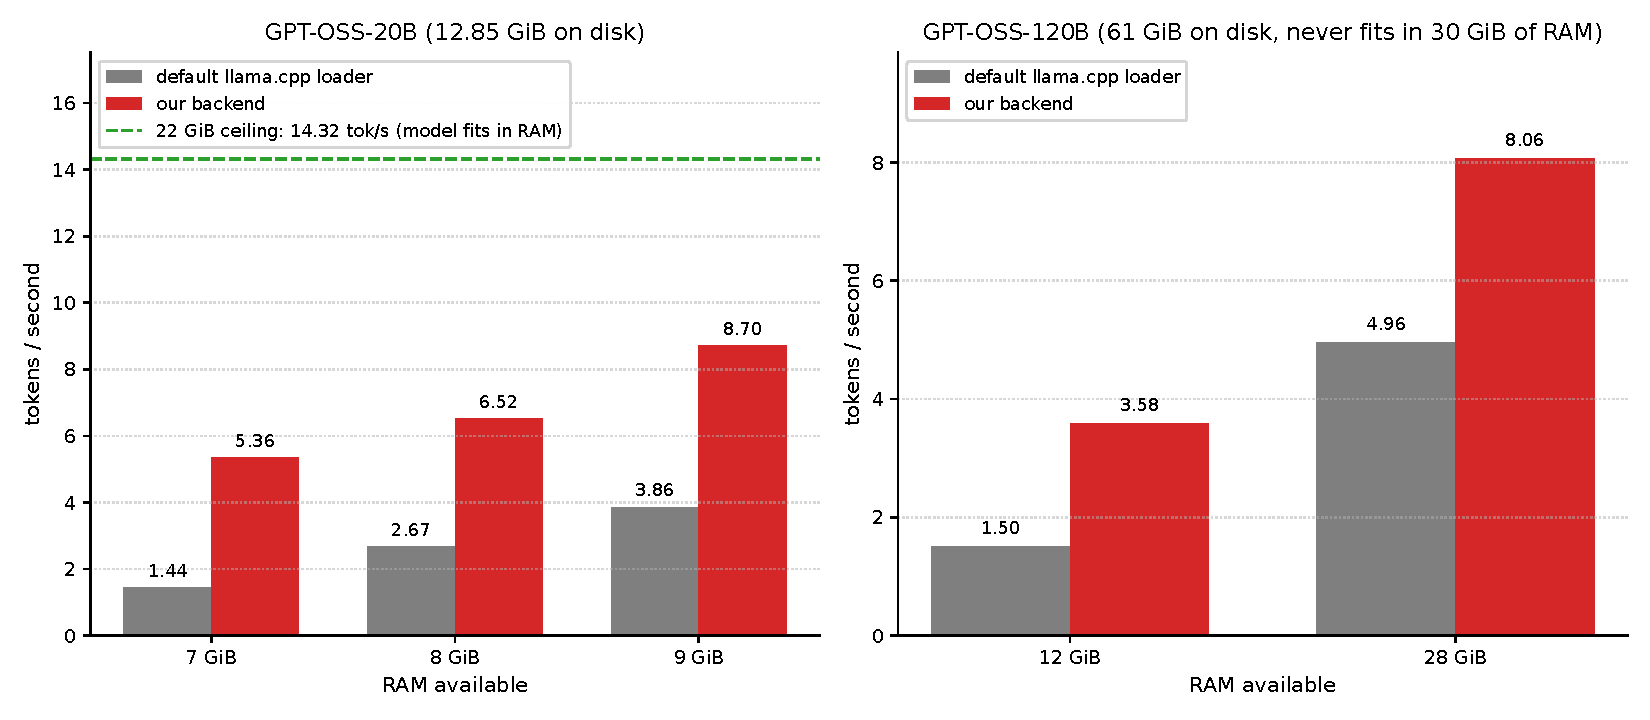
\includegraphics[width=0.85\textwidth]{figures/canon/headline.pdf}
\caption[Decode throughput of the default llama.cpp loader against our backend]{Decode throughput of the default llama.cpp loader (gray) against our backend (red), at three RAM caps for GPT-OSS-20B and two for GPT-OSS-120B. The dashed line on the left panel marks the 14.32~tok/s ceiling reached when GPT-OSS-20B fits entirely in RAM at the 22~GiB cap. GPT-OSS-120B (60.88~GiB on disk) never fits in the 30~GiB of RAM on the test machine, so there is no in-RAM ceiling on the right panel.}
\label{fig:headline}
\end{figure}
